%motivation - representation fairness
Thus far we discussed \nameNS's mechanisms for combating transaction censorship and ensuring fair primary (and committee) election. We now turn to the more subtle procedure of constructing blocks from the pool of pending transactions.

In typical blockchain protocols, nodes (such as Bitcoin's miners) have the freedom to select which transactions to include in their blocks. Normally, when transactions come along with a fee determined by the issuer, this results in a fee market that drives fees unnecessarily high at times of high demand. While we do not elaborate on \nameNS's fee structure, we emphasize that \name is designed such that fees do not play a role in $etx$ selection\footnote{This design choice enables a variety of fee mechanisms e.g., constant fee per transaction, periodic subscription fees, and models in which fees are determined after processing.}. This design choice makes sense when fees are not needed as the main motivation of nodes to include transactions in blocks. Indeed, our presumption in \name is that nodes have inherent interest in processing their own transactions\footnote{For instance, nodes run consumer applications and wish to service their end-users by processing the transactions they issue.}. 
Under these circumstances, the main goal of this section is to describe \nameNS's mechanism for selecting $etx$s in a \emph{fair} manner. Fairness in this regard should be reflected by the blockchain, representing each node according to the proportion of $etx$s she owns\footnote{Under such notion of fairness nodes may be encouraged to artificially produce many self-owned transactions in order to get more block real-estate. Carefully designed fee mechanisms could disincentive such behavior, e.g., paying increased fee for failing transactions.}.

An important aspect in the context of fair sampling is the relation between the rate at which $etx$s are issued and the rate at which they are appended to the blockchain. An epoch at which the \emph{issuance rate} is smaller than the maximal \emph{append rate} (allowed by the system) is relatively easy to analyze---all transactions are processed within a small time frame. A more involved case is when the issuance rate is (temporarily) greater than the append rate. During such epochs, there are many $etx$s pending to be added to the blockchain, and the decision of which $etx$s to include in Eblocks is subject to manipulation. The core aspect of selection fairness is to ensure that the average \emph{waiting time} of an $etx$ depends solely on the number of pending transactions, rather than on its owner node or on any other characteristic.   

In high-load epochs, we adapt a strategy of \emph{correlated sampling} that restricts the freedom a primary has in selecting which $etx$s to include in her Eblock.
%way $etx$s are selected to be included in Eblocks. 
Correlated sampling, considered in~\cite{HashSample1,HashSample2,HashSample3} (see also~\cite{OptCorSampling} for a review and optimality result), refers to the problem in which there are two players having different distributions over the same domain (in our case the set of issued $etx$s) and access to shared randomness (in our case the random seed). Each player wishes to output a single element, sampled according to her distribution while minimizing the probability that the outputs differ. In the work of~\cite{HashSample1}, a MinHash strategy was used for performing correlated sampling for the case that the distributions are uniform over a subset of the domain (analogous to Epools in our setting). In~\cite{hashsamplemultiple}, Rivest applied the MinHash strategy sequentially in order to sample many elements from the domain, possibly with repetitions. However, to the best of our knowledge the scenario of correlated sampling of many elements without repetitions has not been analyzed before.   

%Section structure
Instead of dictating an Eblock construction strategy that might not be aligned with primaries' selfish interests and might be difficult to validate, we suggest an Eblock validation procedure that is better aligned with nodes' interests. In the following section we describe the Eblock validation procedure applied in \name in accordance with the correlated sampling scheme. We then show that strategies with substantial probability of passing validation remain close to the construction dictated by the correlated sampling scheme. Throughout this section we restrict ourselves to high-load epochs by assuming that the total number of pending $etx$s is $\Gamma b$ for some $\Gamma > 1$ (where $b$ is the maximal number of $etx$s in a valid Eblock). 

\subsection{Eblock validation} \label{Validation}
%common ordering of $etx$s in Epool in term $r$.
The \name correlated sampling scheme uses a hash function in order to serialize candidate $etx$s for the next Eblock. The hash function is tweaked with a random seed to eliminate its predictability, yielding a common, random and unpredictable serialization of the $etx$s. Formally, when considering the Eblock in term $r$, the nodes order the pending $etx$s according to the values $H(RS^{r-1},etx)$, and refer to these values as the \textit{hash values} of the $etx$s. We denote $H(etx)$ for brevity. 

%where the dot to the left of $H$ denotes the binary fraction the hash represents, so all hash values are in $[0,1]$. We assume the hash function distributes these values uniformly in $[0,1]$, and conclude that the probability of an $etx$ to be hashed below a given threshold $T\in [0,1]$ is exactly $T$. For brevity we usually write $H(etx)$ rather than $.H(RS^{r-1},etx)$. 

%Introducing locking times
To ensure unpredictability, we introduce the notion of \textit{locking time}. We denote by $EP_i^\tau$ node $i$'s locked Epool at time $\tau$, which is a snapshot of the $etx$s in $i$'s Epool at time $\tau$\footnote{This can be implemented by attaching a timestamp to each $etx$ at the time it was received.}. We denote by $\tau_i'$ the time at which node $i$ revealed $DB^{r-1}$, and define the locking time of node $i$ to be $\tau_i:=\tau_i'-2\Delta$ (recall the definition of $\Delta$ from Sec.~\ref{communication_schemes} as the upper bound on the dissemination time between any pair of nodes).

%upshot of locking times
In the validation procedure, nodes are asked to consider the serialized $etx$s in their Epool at locking time. The choice of $\tau_i$ was made such that nodes cannot quickly tailor $etx$s with low hash values \emph{after} revealing the random seed, but \emph{before} the rest of the network does.  Indeed, due to network latency it could be the case that $RS^{r-1}$ is revealed to some node before the rest of the network---by at most $2\Delta$ time. Without the notion of locking time nodes could have exploited this time to generate and forward tailored $etx$s, detracting from the randomness of the common ordering. Restricting nodes to consider only $etx$s which were known to them prior to time $\tau_i'-2\Delta$ prevents this kind of attack. From now on by writing $EP_i$ we mean $EP_i^{\tau_i}$, unless stated otherwise.

%A primary is asked to include in its Eblock the $b$-minimal hashed $etx$s of its Epool (\textit{$b$-minimal Eblock construction}). Each committee member is asked to validate this selection by comparing the primary's Eblock with the set of lowest hashed $etx$s in its own Epool. The primary's Eblock is validated iff for enough committee members, the intersection of these two sets is large enough.

%The validation conditions are set such that even though different Epools differ slightly due to network latency, correct nodes accept the $b$-minimal construction with overwhelming probability. If, on the other hand, the primary chooses to include in its Eblock $etx$s which are not among its $b$ minimal $etx$s, then this Eblock has a lower probability of passing validation and is more likely to get rejected. 

%Notations and notions we use in the validation procedure

Due to network latency and inherent properties of \nameNS, we cannot expect $EP_i$ and $EP_j$ to be identical, even if $i$ and $j$ are correct nodes. However, as locking times are similar, we may assume a measure of similarity between two correct Epools at locking times.
%\footnote{Entities with ability to predict network timing may conduct an attack that results in correct Epools being largely dissimilar. To mitigate such an attack, $\tau_i$ can be modified to $\tau_i:=\tau_i'-2\Delta-\eta_i$, where $\eta_i$ is locally sampled by $i$ in the range $[0,\Delta]$. This would decouple the predictability of the network from the locking-time procedure.}. 
To model this similarity, we use a probabilistic model satisfying the following property. For any two correct nodes $i,j$ each $etx$ in $EP_i$ is in $EP_j$ with probability at least $\alpha$. We refer to $\alpha$ as the \emph{similarity parameter} of the network.
%\footnote{Notice that this model clearly ignores the fact that an $etx$ which was issued by node $i$ is certainly in $EP_i$. We ignore this fact strictly for brevity.}.

%\red{To model this we consider the set $GP$, which is the \emph{global Epool} of round $r$, defined as $GP = \cup_{i}EP_i^{t_i}$ where the union is done over all correct nodes $i$. The Epools similarity can now be modeled precisely by a simple probabilistic model. $EP_i$ is a random sample of $GP$, containing any $etx$ from $GP$ with probability at least $\alpha$.}

Upon receiving a proposed Eblock, $EB_p$, from primary $p$, correct committee member $i$ validates it by performing the validation procedure presented in Sec.~\ref{Protocol:ValidateEB}. In addition, she checks two conditions regarding the size of the proposed Eblock and the size of its overlap with a set of transactions calculated according to her own Epool. 
We define $T_p$ be the maximal hash of an $etx$ in $EB_p$, i.e., $T_p:=\max\{H(etx)\vert etx\in EB_p\}$. Likewise, we denote by $EB_i' :=\{etx\in EP_i|H(etx)\leq T_p\}$ the set of $etx$s in $EP_i$ with hash values lower than $T_p$, and $b_i:=\max\{|EB_i'|,b\}$. We further denote by $b'$ the size of $EB_p'=\{etx\in EP_p|H(etx)\leq T_p\}$ and say that $EB_p$ was constructed under a $b'$-construction. 
This illustrates the fact that $EB_p$ was selected as a subset of size $b$ among the $b'$ lowest hashed $etx$s in $EP_p$ such that the $b'^{\text{th}}$ $etx$ was included. The setting is illustrated in Fig.~\ref{fig_correlated_sampling}.


\begin{figure}
%[!b]%[!ht]
	\centering
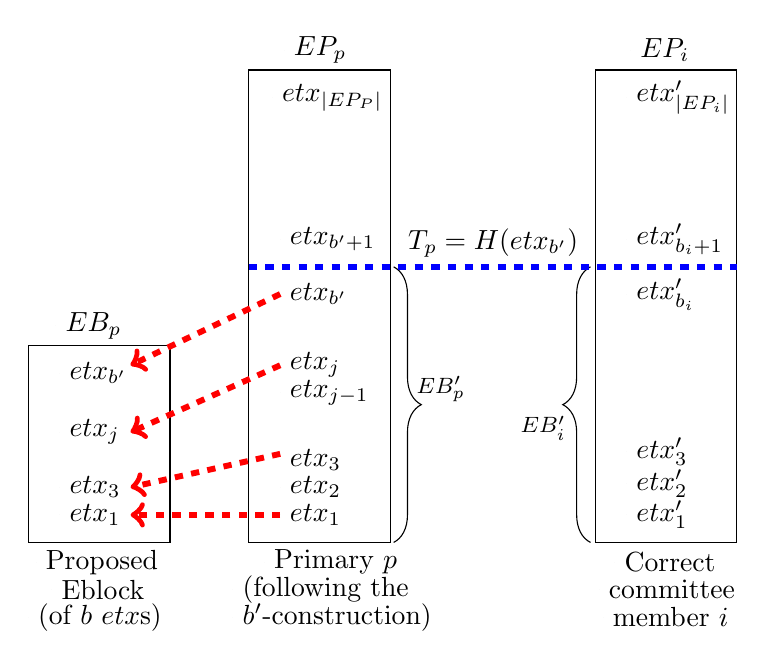
\begin{tikzpicture}
\tikzstyle{every loop}=[]
\draw (0,0) rectangle (1.8,2.5);
\draw (2.8,0) rectangle (4.6,6);
\draw (7.2,0) rectangle (9,6);

\filldraw[black] (0.1,-0.25) circle (0pt) node[anchor=west] {Proposed};
\filldraw[black] (0.3,-0.6) circle (0pt) node[anchor=west] {Eblock};
\filldraw[black] (0,-0.95) circle (0pt) node[anchor=west] {(of $b$ $etx$s)};
\filldraw[black] (3.00,-0.25) circle (0pt) node[anchor=west] {Primary $p$};
\filldraw[black] (2.60,-0.6) circle (0pt) node[anchor=west] {(following the};
\filldraw[black] (2.60,-0.95) circle (0pt) node[anchor=west] {$b'$-construction)};
\filldraw[black] (7.45,-0.25) circle (0pt) node[anchor=west] {Correct};
\filldraw[black] (7.25,-0.6) circle (0pt) node[anchor=west] {committee};
\filldraw[black] (7.30,-0.95) circle (0pt) node[anchor=west] {member $i$};


\filldraw[black] (0.35,2.75) circle (0pt) node[anchor=west] {$EB_p$};
\filldraw[black] (3.25,6.25) circle (0pt) node[anchor=west] {$EP_p$};
\filldraw[black] (7.65,6.25) circle (0pt) node[anchor=west] {$EP_i$};

\filldraw[black] (0.4,0.35) circle (0pt) node[anchor=west] {$etx_{1}$};
\filldraw[black] (0.4,0.7) circle (0pt) node[anchor=west] {$etx_{3}$};
\filldraw[black] (0.4,1.4) circle (0pt) node[anchor=west] {$etx_{j}$};
\filldraw[black] (0.4,2.15) circle (0pt) node[anchor=west] {$etx_{b'}$};
%\filldraw[black] (0.5,5.65) circle (0pt) node[anchor=west] {$etx_{|EP_P|}$};

\filldraw[black] (3.2,0.35) circle (0pt) node[anchor=west] {$\boldsymbol{etx_{1}}$};
\filldraw[black] (3.2,0.7) circle (0pt) node[anchor=west] {$etx_{2}$};
\filldraw[black] (3.2,1.05) circle (0pt) node[anchor=west] {$\boldsymbol{etx_{3}}$};
\filldraw[black] (3.2,1.9) circle (0pt) node[anchor=west] {$etx_{j-1}$};
\filldraw[black] (3.2,2.25) circle (0pt) node[anchor=west] {$\boldsymbol{etx_{j}}$};
\filldraw[black] (3.2,3.15) circle (0pt) node[anchor=west] {$\boldsymbol{etx_{b'}}$};
\filldraw[black] (3.2,3.85) circle (0pt) node[anchor=west] {$etx_{b'+1}$};
\filldraw[black] (3.1,5.65) circle (0pt) node[anchor=west] {$etx_{|EP_P|}$};

\draw [decorate,decoration={brace,amplitude=10pt,mirror},xshift=4pt,yshift=0pt]
(4.5,0) -- (4.5,3.5) node [black,midway,xshift=0.6cm, yshift=0.2cm] 
{\footnotesize $EB'_p$};

\filldraw[black] (7.6,0.35) circle (0pt) node[anchor=west] {$etx'_{1}$};
\filldraw[black] (7.6,0.75) circle (0pt) node[anchor=west] {$etx'_{2}$};
\filldraw[black] (7.6,1.15) circle (0pt) node[anchor=west] {$etx'_{3}$};
\filldraw[black] (7.6,3.15) circle (0pt) node[anchor=west] {$etx'_{b_i}$};
\filldraw[black] (7.6,3.85) circle (0pt) node[anchor=west] {$etx'_{b_i+1}$};
\filldraw[black] (7.6,5.65) circle (0pt) node[anchor=west] {$etx'_{|EP_i|}$};

\draw [decorate,decoration={brace,amplitude=10pt},xshift=4pt,yshift=0pt]
(7.0,0) -- (7.0,3.5) node [black,midway,xshift=-0.6cm, yshift=-0.3cm] 
{\footnotesize $EB'_i$};

\filldraw[black] (4.7,3.8) circle (0pt) node[anchor=west] {$T_p = H(etx_{b'})$};
\draw [-,dashed,thick, blue, line width=0.75mm] (2.8,3.5) to  (9,3.5);

\draw [->,dashed,thick, red, line width=0.75mm] (3.2,0.35) to (1.3,0.35);  
\draw [->,dashed,thick, red, line width=0.75mm] (3.2,1.125) to (1.3,0.7);  
\draw [->,dashed,thick, red, line width=0.75mm] (3.2,2.25) to (1.3,1.4);  
\draw [->,dashed,thick, red, line width=0.75mm] (3.2,3.155) to (1.3,2.25); 



 \path[]
 ;
\end{tikzpicture}
 \caption{Illustration of the correlated sampling validation process. In each Epool, $etx$s are sorted based on their hash values. A threshold $T_p$ is determined by the maximal hash value of an $etx$ in the EBlock $EB_p$ proposed by the primary $p$. A correct committee member $i$ examines the overlap between $EB_p$ and the set of $etx$s in $EP_i$ which hash below $T_p$.	}\label{fig_correlated_sampling}
\end{figure}






% \begin{figure}
% %[!b]%[!ht]
% 	\centering
% \begin{tikzpicture}
% \tikzstyle{every loop}=[]
% \draw (0,0) rectangle (1.8,2.5);
% \draw (2.8,0) rectangle (4.6,6);
% \draw (7.2,0) rectangle (9,6);

% \filldraw[black] (0.1,-0.25) circle (0pt) node[anchor=west] {Proposed};
% \filldraw[black] (0.3,-0.55) circle (0pt) node[anchor=west] {block};
% \filldraw[black] (0,-0.85) circle (0pt) node[anchor=west] {(of $b$ $etx$s)};
% \filldraw[black] (3.00,-0.25) circle (0pt) node[anchor=west] {Leader $l$};
% \filldraw[black] (7.20,-0.25) circle (0pt) node[anchor=west] {Verifier};
% %\filldraw[black] (7.30,-0.55) circle (0pt) node[anchor=west] {member $i$};


% \filldraw[black] (0.5,2.75) circle (0pt) node[anchor=west] {$B_l$};
% \filldraw[black] (3.5,6.25) circle (0pt) node[anchor=west] {$P_l$};
% \filldraw[black] (7.5,6.25) circle (0pt) node[anchor=west] {$P_i$};

% \filldraw[black] (0.4,0.35) circle (0pt) node[anchor=west] {$etx_{1}$};
% \filldraw[black] (0.4,0.7) circle (0pt) node[anchor=west] {$etx_{2}$};
% \filldraw[black] (0.4,1.4) circle (0pt) node[anchor=west] {$etx_{j}$};
% \filldraw[black] (0.4,2.15) circle (0pt) node[anchor=west] {$etx_{b}$};
% %\filldraw[black] (0.5,5.65) circle (0pt) node[anchor=west] {$etx_{|EP_P|}$};

% \filldraw[black] (3.2,0.35) circle (0pt) node[anchor=west] {$\boldsymbol{etx_{1}}$};
% \filldraw[black] (3.2,0.7) circle (0pt) node[anchor=west] {$\boldsymbol{etx_{2}}$};
% \filldraw[black] (3.2,1.05) circle (0pt) node[anchor=west] {$\boldsymbol{etx_{3}}$};
% \filldraw[black] (3.2,1.9) circle (0pt) node[anchor=west] {$\boldsymbol{etx_{j-1}}$};
% \filldraw[black] (3.2,2.25) circle (0pt) node[anchor=west] {$\boldsymbol{etx_{b}}$};
% \filldraw[black] (3.2,3.15) circle (0pt) node[anchor=west] {$etx_{b'}$};
% \filldraw[black] (3.2,3.85) circle (0pt) node[anchor=west] {$etx_{b'+1}$};
% \filldraw[black] (3.1,5.65) circle (0pt) node[anchor=west] {$etx_{|P_l|}$};

% \draw [decorate,decoration={brace,amplitude=10pt,mirror},xshift=4pt,yshift=0pt]
% (4.5,0) -- (4.5,2.5) node [black,midway,xshift=0.6cm, yshift=0.2cm] 
% {\footnotesize $B'_l$};

% \filldraw[black] (7.6,0.35) circle (0pt) node[anchor=west] {$etx'_{1}$};
% \filldraw[black] (7.6,0.7) circle (0pt) node[anchor=west] {$etx'_{2}$};
% \filldraw[black] (7.6,1.05) circle (0pt) node[anchor=west] {$etx'_{3}$};
% \filldraw[black] (7.6,3.15) circle (0pt) node[anchor=west] {$etx'_{b_i}$};
% \filldraw[black] (7.6,3.85) circle (0pt) node[anchor=west] {$etx'_{b_i+1}$};
% \filldraw[black] (7.6,5.65) circle (0pt) node[anchor=west] {$etx'_{|P_i|}$};

% \draw [decorate,decoration={brace,amplitude=10pt},xshift=4pt,yshift=0pt]
% (7.0,0) -- (7.0,2.5) node [black,midway,xshift=-0.6cm, yshift=-0.3cm] 
% {\footnotesize $B'_i$};

% \filldraw[black] (4.7,2.8) circle (0pt) node[anchor=west] {$T = H(etx_{b})$};
% \draw [-,dashed,thick, blue, line width=0.75mm] (0,2.5) to  (9,2.5);

% \draw [->,dashed,thick, red, line width=0.75mm] (3.2,0.35) to (1.3,0.35);  
% \draw [->,dashed,thick, red, line width=0.75mm] (3.2,1.125) to (1.3,1.125);  
% \draw [->,dashed,thick, red, line width=0.75mm] (3.2,2.25) to (1.3,2.25);  
%\draw [->,dashed,thick, red, line width=0.75mm] (3.2,3.155) to (1.3,2.25); 



%  \path[]
%  ;
% \end{tikzpicture}
% \end{figure}

Under these notations, the validation checks (in the context of selection fairness) performed by correct node $i$ upon receiving a proposed Eblock, $EB_p$ (from primary $p$), are:
\begin{enumerate}
	\item $|EB_p|=b$ \label{validiation_condition_1}
	\item $|EB_p\cap EB_i'|\geq \beta_{\alpha}(b_i)$ for $\beta_{\alpha}(b_i) :=  \alpha b_i-\sqrt{10 b_i}$ \label{validiation_condition_2}
\end{enumerate}

\noindent The second condition encourages primaries to construct Eblocks with low $b'$. The minimal value of $b'$ is $b$; in the event that the value of $b'$ is in fact $b$, the selection scheme is perfectly fair. Intuitively, a larger $b'$ allows the primary more freedom in the selection of $EB_p$ (rather than selecting it as the $b$ minimal $etx$s). However, since we can expect $|EB_p'| \approx  |EB_i'|$, large $b'$ yields large $b_i$ and accordingly large $\beta_\alpha(b_i)$, reducing the chances of $EB_p$ to pass validation. $\beta_\alpha(b_i)$ is the maximal value for which Eblocks constructed with $b'=b$ pass validation w.o.p., as implied by Hoeffding's bound. This is shown formally in the next section.

% Notice that the larger $|EB_p'\setminus EB_p|=b'-b$ is, the more freedom the primary had in selecting which $etx$s to include in $EB_p$. Since Epools similarity results in $|EB_p'|\sim |EB_i'|$

% $EB_p$ If $EB_p$ is indeed the $b$-minimal $etx$s of $EP_p$, then $EB_p=EB_p'$. It is achieved since on the one hand, $|EB_p\cap EB_i'|$ should be roughly $\alpha b$. Thus, if $b_i\sim b$ then $EB_p$ should pass this validation. On the other hand, $|EB_i'|\sim |EB_p'|$
% when $b'\ge b$ then $T_p'\ge T_i$ and the validation condition becomes $|EB_p'\cap EB_i'|\ge \gamma(b_i)b_i$. Both sides of this inequality grow with $T_p'$, but while the left hand side grows slowly, and is bounded by $b$, the right hand grows faster and is effectively un

% is that if $EB_p$ is composed of the $b$-minimal $etx$s in $EP_p$, then $EB_p=EB_P'$. Since we can expect $EB_p'$ and $EB_i'$ to be quite similar to one another, $EB_p\cap EB_i'$ approximates 

% To formulate the conditions checked in the validation procedure, we introduce the following notions and notations:
% \begin{itemize}
% 	\item $T_p':=max\{H(etx)\vert etx\in EB_p\}$.   \item $EB_p':=\big|\{etx\in EP_p|H(etx)\leq T_p'\}\big|$. We further denote $b':=|EB_p'|$, and note that $EB_p\subset EB_p'$ and is of size $b$. 
% 	\item $EB_i':=\{etx\in EP_i|H(etx)\leq T_p'\}$. We denote $b_i':=|EB_i'|$.
%     \item $EB_i$ is the set of $b$-minimal $etx$s in $EP_i$. 
%     \red{We denote by $T_i$ the maximal hash value of an $etx$s from $EB_i$.}
% \end{itemize}
% We define $b_i:=b_i'=|EB_i'|$ in case $T_i<T_p'$, and $b_i=b=|EB_p|$ otherwise. Notice that in case $T_i<T_p'$, it holds that $EB_i\subset EB_i'$ and $b_i\ge b$.

%intuition for validation conditions 
% We wish to give some intuition regarding the second validation condition. Consider the construction in which the Eblock contains exactly the $b$ $etx$s with lowest hash values in $EP_p$. I.e., this is a $b$-minimal construction. This construction emulates a perfect random construction in terms of the owner nodes representation. Our validation condition is set to check that $EB_p$ does not deviate from this construction by a lot. 
% The way this is done is the following. In the $b$-minimal construction, $T_p'=T_p$, and $EB_p=EB_p'$. In this case, we can expect $b_i'$ to be roughly $b$. Node $i$ should also expect $EP_p$ to contain at least an $\alpha$-fraction of $EB_i'$, which are roughly $\alpha b_i'$. If this is the case,If $EB_p$ was indeed constructed using the $b$-minimal construction then $EB_p\cap EB_i'=EP_p\cap EB_i'$, and so, on average $|EB_p\cap EB_i'|\sim \alpha b_i$ (recall in this case $b_i:=|EB_i'|$). The purpose of the validation condition is to make sure that this more or less the case.

% \textbf{Tradeoff in the selection of $\pmb{\beta}$}: Setting the function $\beta$ is a critical task. On the one hand, a large $\beta(b_i)$ guarantees solid correlated sampling resulting in \emph{representation fairness}, which is simply to say that nodes' representation in each Eblock is similar to their relative part in the overall issued $etx$s. On the other hand, the larger $\beta(b_i)$ is, committee members are more strict in validating Eblocks. Thus, potential differences between Epools of correct nodes might result in Eblocks being rejected often, and guaranteeing liveness becomes more difficult. %\red{further explanation needed, I would rephrase}. 

\subsection{Liveness under $b$-construction} \label{Liveness}
%The problem in Helix terms
The extra validation process dictated by the correlated sampling scheme bears risk to the liveness of the protocol. Blocks that would have passed validation might get rejected once correlated sampling validation is enforced. We thus prove that an Eblock compliant with the $b$-construction passes validation of any correct committee member w.o.p.

\begin{claim} [Liveness under $b$-construction.] \label{liveness} Let $EB_p$ be an Eblock constructed according to the $b$-construction, $i$ be a correct committee member. Then, $EB_p$ passes $i$'s validation w.o.p. (under the assumption that $\alpha$ bounds from below the similarity parameter of the network)
\end{claim}
\noindent We use the following lemma.
\begin{lemma}
For two correct nodes $k,l$ and a general set $A\subset EP_l$, $|A\cap EP_k|>\beta_\alpha(|A|)$ with probability greater then $1-2\exp(-20)$, where $\beta_\alpha(x):=\alpha x-\sqrt{10x}$.
\end{lemma}
\begin{proof}
Denote $Y:=|A\cap EP_k|$. We can write $Y=\sum_{etx\in A}Y_{etx}$, where $Y_{etx}$ are indicator random variables, 
\begin{equation*}
    		Y_{etx} =	
		    \begin{cases}
    			  1  &\mbox{if }  etx\in EP_k \\
     			  0  &\mbox{otherwise}
		     \end{cases}
  	\end{equation*}
By definition, these random variables are i.i.d. Bernoulli variables, with success probability (at least) $\alpha$. This is true from the similarity assumption. By Hoeffding's inequality, for any $\delta \ge 0$
$$Pr \left( \frac{1}{|A|}|Y-\mathbb{E}(Y)| >\delta \right) \leq 2\exp(-2|A|\delta^2)$$
%Bounding the above probability by $2\exp(-20)$, we derive an inequality $2|A|\delta^2 \ge 20\iff \delta \ge \sqrt{\frac{10}{|A|}}$.
The expected value of $Y$ is bounded from below by $\alpha |A|$, thus taking $\delta=\sqrt{\frac{10}{|A|}}$ and plugging this into the left-hand side of Hoeffding's inequality, we get that with probability $>1-2\exp(-20)$ 
\begin{equation*}\begin{split}|A\cap EP_i|= Y&>\mathbb{E}(Y)-|A|\delta\\ &\ge \alpha\cdot |A|-\sqrt{10|A|}=:\beta(|A|) \qedhere
\end{split}\end{equation*} 
\end{proof}

\noindent We now turn to prove claim~\ref{liveness}. 
\begin{proof}
Node $i$'s validation comprises of two checks. Check number~\ref{validiation_condition_1} is that $|EB_p|=b$, which passes with probability $1$. For clarity of the proof, we break check number~\ref{validiation_condition_2} into two:
\begin{enumerate}
	\item[2.1] $|EB_p\cap EB_i'|\geq \beta_{\alpha}(b)$ 
	\item[2.2] $|EB_p\cap EB_i'|\geq \beta_{\alpha}(|EB_i'|)$
\end{enumerate}
For $2.1$, take $A=EB_p\subset EP_p$. For a correct primary, this is simply a general random set of transactions of size $b$. The above lemma can be used as $|EB_p\cap EB_i'|=|EB_p\cap EP_i|$, yielding that the probability for failing this condition is at most $2\exp(-20)$.
The argument for condition $2.2$ is similar, only this time $A=EB_i'\subset EP_i$ and we use the equality $|EB_i'\cap EB_p |=|EB_i'\cap EP_p|$. The latter equality is derived from the assumption that $EB_p$ is a $b$-construction, which implies $EB_p=EB_p'=\{etx\in EP_p|H(etx)\leq T_p\}$. Now, the equality is easily derived from the definition of $EB_i'$.
%Combining the probabilities for $2.1$ and $2.2$ concludes the proof. \red{conditions 2.1 and 2.2 merge into one condition only when $\beta_\alpha(b_i)$ is a monotonically increasing function which is true only when $b_i\geq2.5/\alpha^2$, note that for $\alpha\geq0.5$, $b_i$ should be $\geq10$.}
\end{proof}

 
%Proof of claim (formal)
The claim establishes the fact that a primary following the $b$-construction would pass validation w.o.p., thus keeping the protocol live. 
In the next section we generalize the analysis above, considering Eblocks admitting $b'$-constructions for $b'>b$.




% \begin{tikzpicture} \label{graph11}
%   \begin{axis}[ 
%     xlabel={probability for passing validation ($q$)},
%     ylabel={maximal $etx$ (b'(q))$/1000$},
%     xmin=0.5, xmax=1,
%     ymin=1090, ymax=1120,
%     xtick={0.5,0.6,0.7,0.8,0.9,0.95},
%     ytick={1100,1105,1110,1115,1120}
%   ] 
%   \addplot [
%     color=blue,
%     mark=square,
%     ]
%     coordinates {
%     (0.9377,1100)(0.9053,1102)(0.8693,1104)(0.8371,1106)(0.7833,1108)(0.7231,1110)(0.6578,1112)(0.5979,1114)
%     }
%     \addplot [
%     color=red,
%     mark=square,
%     dashed
%     ]
%     coordinates {
%     (0.986,0.97, 0.948, 0.92, 0.880.8199999999999998
% 0.7199999999999998
% 0.5199999999999995
%     };
%   \end{axis}
% \end{tikzpicture}
% \red{TABLE, GRAPH?}
% Before we continue we note that while the values $\beta(b_i) = \alpha^2b_i-\sqrt{10b_i}$ and $\beta'=\alpha b_i-\sqrt{10b_i}$ are functions of the similarity bound $\alpha$ and the block size $b$, a lower bound on the value of $\beta$ holds in practical settings.
% %b = 200 or 2000 ??
% For $\alpha \ge 0.95$ and $b \ge 2000$ it satisfies $\beta \ge 0.83$. 
% Table~\ref{tab:table1} illustrates the values of $\beta$ for $\alpha \in \{0.90,0.95\}, b \in \{1000,2000,5000\}$. Values of $\beta$ are also presented 
% in Fig.~\ref{fig:beta_vs_alpha}.  
 
% \begin{table}[h!]
%   \begin{center}
%     \caption{$\beta$ calculated for different values of $\alpha$ and $b$}
%     \label{tab:table1}
%     \begin{tabular}{c|c|c|c} % <-- Alignments: 1st column left, 2nd middle and 3rd right, with vertical lines in between
%       $b$ & $\alpha$ &$\alpha ^2$ &  $\beta$ \\
%       \hline
%       1000&0.90 &0.8100&0.7100\\
%       1000&0.95 &0.9025&0.8025\\
%       2000&0.90 & 0.8100 & 0.7393\\
%       2000&0.95 &0.9025&0.8317\\
%       5000&0.90 & 0.8100 & 0.7653\\
%       5000&0.95 &0.9025&0.8578\\
%     \end{tabular}
%   \end{center}
% \end{table}


% \begin{figure}[!t]%[!ht]
% \centering
% \begin{tikzpicture}
% \begin{axis}[
% xmode=log,
%    xlabel={block size $b$},
%    ylabel={$\beta$},
%     %ylabel={$\phi(x)$},
%     xmin=1000, xmax=50000,
%     ymin=0, ymax=1,
%     xtick={1000, 2000, 5000, 10000, 20000,50000},
%     xticklabels={1K, 2K, 5K, 10K, 20K,50K},
%     ytick={0,0.2,0.4,0.6,0.8,1},
%     legend pos=north west,
%     ymajorgrids=true,
%     grid style=dashed,
%     height = 6.2cm,
%     width = 0.50*\textwidth,
%  %   line width=1.6pt,
% %]
%                 legend style={at={(0.65,0.05)},anchor=south west,font=\scriptsize},
%                 label style={font=\footnotesize}, grid=both];
%             %\addplot [black,mark=x] table [x={chi}, y={cooperative}] {\resfirsta};
%         \addplot[% only marks, mark=square,  black,mark=
%    color=red,mark=*,scale=10, line width=1pt,mark options={line width=0.9pt,draw=red,fill=red}]
%     coordinates {
% (1000, 0.8025) (1400, 0.8179845745271483) (2000, 0.8317893218813452) (3000, 0.8447649730810374) (5000, 0.8577786404500042) (7000, 0.8647035526990773)(10000, 0.8708772233983162) (14000, 0.8757738758087575) (20000, 0.8801393202250021) (35000, 0.8855969149054297) (50000, 0.8883578643762691)
%     };
%     \addlegendentry{$\alpha = 0.95$};
%     \addplot[% only marks, mark=square,  black,mark=
%    color=green,mark=triangle,%dotted, 
%    scale=10, line width=1pt,mark options={line width=0.9pt,draw=green,fill=green}]
%     coordinates {
%         (1000, 0.7100000000000001) (1400, 0.7254845745271484) (2000, 0.7392893218813453) (3000, 0.7522649730810375) (5000, 0.7652786404500043) (7000, 0.7722035526990774) (10000, 0.7783772233983163) (14000, 0.7832738758087576) (20000, 0.7876393202250022) (35000, 0.7930969149054298) (50000, 0.7958578643762692)
%     };
%     \addlegendentry{$\alpha = 0.9$};
% \addplot[% only marks, mark=square,
%    color=gray,mark=square,scale=10, line width=1pt,mark options={line width=0.5pt,draw=gray,fill=gray}]
%     coordinates {
%    (1000, 0.5400000000000001) (1400, 0.5554845745271485) (2000, 0.5692893218813454) (3000, 0.5822649730810375) (5000, 0.5952786404500043) (7000, 0.6022035526990774) (10000, 0.6083772233983163) (14000, 0.6132738758087577) (20000, 0.6176393202250022) (35000, 0.6230969149054298) (50000, 0.6258578643762692)
%     };
%     \addlegendentry{$\alpha = 0.8$};
% \end{axis}
% \end{tikzpicture}
% \caption{The value of $\beta$ calculated for different values of $\alpha$ and $b$}
% \label{fig:beta_vs_alpha}
% \end{figure}
